\documentclass[letter,11pt]{article}

\usepackage[spanish]{babel}
\usepackage[utf8]{inputenc}
\usepackage{indentfirst}
\usepackage[hidelinks]{hyperref}
\usepackage{float}
\usepackage{array}
\usepackage{subcaption}
\usepackage{setspace}
\setlength{\parindent}{0in}
\usepackage{listings}
\usepackage{csquotes}
\usepackage{amsmath, amssymb, amsfonts, latexsym, mathrsfs}
\usepackage{graphicx}
\usepackage{listings}

% Interlineado
\usepackage{setspace}
\spacing{1.5}

% Márgenes
\usepackage[top = 2.3cm, bottom = 2.3cm, left = 2.6cm, right = 2.6cm]{geometry}


% Número de página
\usepackage{fancyhdr}
\pagestyle{fancy}
\rhead[]{}
\lhead[]{}
\renewcommand{\headrulewidth}{0pt}
\rfoot[]{\thepage}
\cfoot[]{}
\begin{document}

% PORTADA
\thispagestyle{empty} 

\begin{center} \LARGE{UNIVERSIDAD NACIONAL AUTÓNOMA DE MÉXICO} \\[0.5cm] \Large{FACULTAD DE INGENIERÍA}\\[0.40cm] \large{ FACULTAD DE INGENIERÍA} \end{center}
\begin{figure}[htb] 
    \centering 
    
\includegraphics[scale=.6]{protecologo.jpg} 
\end{figure}
\begin{center} \large{\bf Proyecto Final}\\ \vspace{.25cm} { \Large \bfseries \underline{Terminal personalizada}} \\ \end{center}
\large{\bf Curso: } Linux\\
\large{\bf Integrantes: }
    \begin{itemize}
        \item Iván Antonio Fernández Cano
    \end{itemize}
\large{\bf Generación prebrecarios:} 45\\
\begin{center} 
    \Large \textsc{Fecha de entrega} \\
    \Large \textsc{22 DE SEPTIEMBRE DE 2023} 
\end{center}

\tableofcontents
\setcounter{tocdepth}{4}

\newpage

\section{Introducción}
Este trabajo en lo personal me ayudó muchísimo a expandir mis conocimientos de Linux y de programación en general.
A lo largo de este, se involucraron conceptos que habíamos visto en el tiempo que duró el curso y además otros cuantos
que tuve que investigar por mi cuenta, y de los cuales, explicaré en un momento.\\

\newpage

\section{Desarrollo del proyecto}

\subsection{Antes de empezar...}
La metodología que fui siguiendo para elaborar el proyecto fue cambiando conforme avanzaba en este. Decidí primero
realizar los scripts de los comandos por separada, mi idea era que una vez que ejecutaran de manera correcta, podría pasar ahora sí a la parte del diseño que involucraría juntar todos estos comandos para dar vida a lo que sería la terminal
personalizada. Con el paso de los días, me fue inevitable comenzar a desarrollar como tal el menú principal y la lógica
para que el usuario pudiera ejecutar cada uno de estos comandos como se indicó en la rúbrica.\\

Un común denominador en la mayoría de los scripts, fue el uso de ASCII arts simplemente para una mejor presentación
en la terminal, ya que toda la interacción con el programa se hace mediante la línea de comandos. Mediante el uso de una función llamada 'title()', en cada uno de los scripts se manda a llamar al inicio para que se despliegue el título
del comando.

\subsection{Ventana de inicio de sesión}
En este script realicé un menú principal que me permitiera iniciar sesión para así dar acceso al CLI (Command Line Interface). \\
Para que el usuario pueda acceder al CLI, tiene que forzozamente iniciar sesión al ingresar la opción 1, en donde con el comando 'read', se lee su nombre de usuario. Aquí es donde tengo la primera condición importante dentro de este script.\\

\begin{lstlisting}[language=sh, label={lst:shellscript}, basicstyle=\small]
if getent passwd "$username" > /dev/null; then
\end{lstlisting}

La condicional anterior, primero ejecuta el comando 'genent passwd' que nos brinda el contenido del archivo 'passwd' del sistema. Recordemos que en este archivo es donde podemos ver los usuarios registrado en el sistema operativo anfitrión. Además, enseguida hacemos uso de la variable 'username', que es el nombre de usuario que introdujo el usuario previamente. Lo anterior para que nos muestre la información exclusiva de la cadena que ingresó el usuario activo. Después de eso utilicé el operador '>' para direccionar la salida del comando anterior al directorio '/dev/null', esto me sirvió mucho ya que por lo que entendí es una especie de directorio en donde se guarda basura del sistema, o bien, información que no es relevante y que es descartable y sirve simplemente para no mostrar su contenido en pantalla. ¿Por qué nos sirve esto para verificar si un usuario existe en el sistema? Al estar dentro de la condición if, si el comando logra encontrar la información del 'username' ingresado, entonces se evalúa como verdadera y significa que el usuario existe en el sistema. Si no existe, entonces en el 'else' le indicamos al usuario que no existe el username en el sistema.\\

Una vez que ya comprobamos la existencia del usuario en el sistema, ingresa su contraseña. Aquí utilice la bandera -n para que no se viera la entrada de la contraseña del usuario, con fines más de seguridad como pasa cuando ejecutamos alguna opción como superusuario. La siguiente condición nos ayuda a verificar si la contraseña ingresada coincide con la registrada en el archivo shadow del sistema.

\begin{lstlisting}[language=sh, label={lst:shellscript}, basicstyle=\small]
if ! echo "$password" | su "$username" -c 'echo " "' 2> /dev/null; then
\end{lstlisting}

Primero direcciono la contraseña ingresada por el usuario, y con ayuda del operador tubería, entonces es cuando mando a llamar a comando 'su' que permita ejecutar a su vez el comando echo que imprime un espacio. Es muy importante la bandera -c ya que hace que no cambie de usuario como tal, sino que simplemente permite ejecutar el comando siguiente. La expresión 2> redirecciona cualquier salida de error del comando 'su' al directorio basura. En resumen, si la contraseña coincide con la ingresada, entonces el 'echo' de la bandera -c se ejecutará y por ende significa que las contraseñas coincide, si no se ejecuta de manera correcta entonces significa que las contraseñas no coinciden. \\

Con ayuda de una variable bandera me apoyo para verificar que lo anterior que haya logrado con éxito o no, es por eso que si las contraseñas coinciden, ahora sí ejecuto el archivo 'main.sh', permitiéndole el acceso al usuario al CLI.

\begin{figure} 
    \centering
    \caption{Usuario inexistente y contraseña incorrecta}
    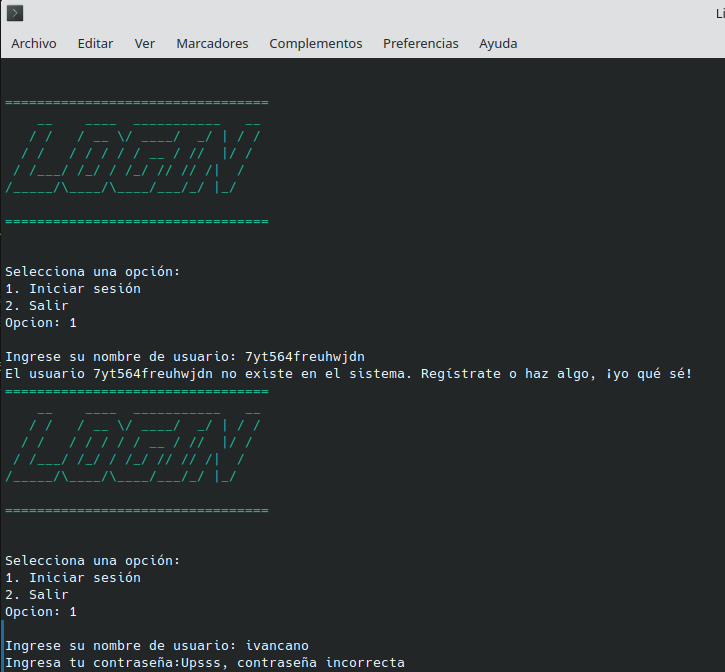
\includegraphics[scale=.6]{sesion1.png} 
\end{figure}

\begin{figure} 
    \centering 
    \caption{Inicio de sesión exitoso}
    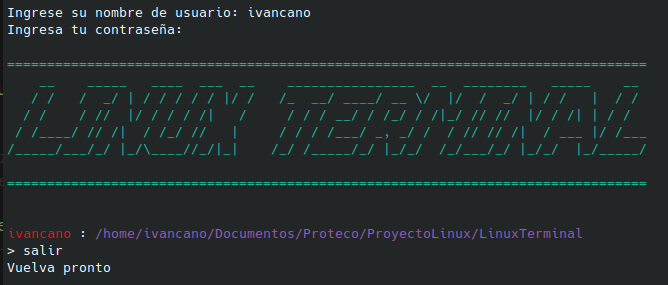
\includegraphics[scale=.6]{sesion2.png} 
\end{figure}


\newpage
\subsection{Línea de comandos del sistema}

Una vez que se verifica el usuario y la contraseña, cuando son correctas se accede al CLI. En este primero que nada hacemos que el parámetro de \$1 sea el username, esto es posible solo si la contraseña fue correcta. \\
Utilicé una función para desplegar un mensaje en pantalla cuando el usuario trata de interrumpir el proceso con ctrl+z ó en su defecto con ctrl+c. También al principio del script declaré un arreglo, que contiene más que nada los comandos personalizados y me ayudan para verificar la entrada del usuario.\\

Tenemos el bucle principal en donde tuve problemas al inicio en la comparación de cadenas. Finalmente me decanté por la opción de comparar una cadena (que en este caso es el comando introducido por el usuario) con la expresión regular que está a la derecha del operador '=~', que es simplemente salir. Así permite salir al usuario de la línea de comandos.\\

Posteriormente llega la parte del comando trap, que es el que me permite ejecutar una acción en dado caso de que detecte alguna señal. Las señales con mecanismos de comunicación entre el sistema operativo y el kernel, ayudan a verificar o ejecutar ciertos eventos en procesos de ejecución. El comando trap, como su traducción me lo indica, me permite hacer una trampa para que el sistema atrape la señal en cualquier momento que se ejecute dentro del script. Las señales de ctrl+z y ctrl+c se representan mediante los nombres SIGTSTP y SIGINT, respectivamente, por lo que cada vez que usuario introduzca estas señales, en lugar de interrumpirse el proceso de la terminal personalizada, manda a llamar a la función malo, que imprime un mensaje en pantalla tratando de ser gracioso jaja ): \\

\begin{figure} 
    \centering 
    \caption{Uso del comando trap}
    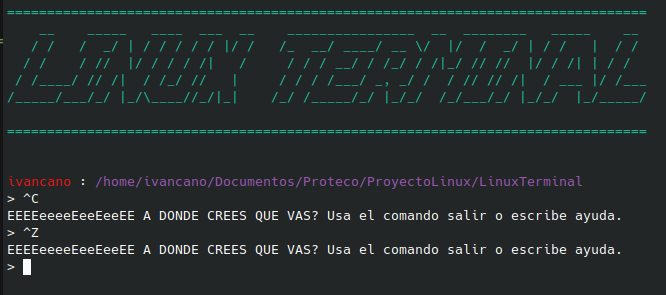
\includegraphics[scale=.6]{trap.png} 
\end{figure}

Para la impresión de títulos y ciertas líneas a lo largo de la terminal, utilicé algunos códigos de colores que tiene Linux para darle un formato más vistoso a la salida. \\
A continuación, viene una condicional que es muy importante para la verificación de los comandos personalizados, y es más que nada la utilización de una búsqueda con el comando grep en el arreglo para verificar si el comando que ingreso el usuario se encuentra presente en el arreglo. Al fin de cuentas es una arreglo de cadenas, en donde lo uso como referencia verificar si un comando personalizado existe o no, y en donde en resumen, el operador de triple menor que, me permite utilizar a mi arreglo como si fuera un archivo de texto (no tal cual pero es una analogía acertada teniendo en cuenta que sus elementos son cadenas de texto) y se lo redirecciono al comando grep para que busque el comando.\\

\begin{lstlisting}[language=sh, label={lst:shellscript}, basicstyle=\small]
if grep -q "$comando" <<< "${misComandos[@]}"; then
\end{lstlisting}

De la anterior manera, puedo acceder a un menú switch case en donde en dado caso de que el se haya ingresado correctamente el comando personalizado lo ejecuta.\\
Si el grep no encontró el comando en mi arreglo inicial, procede entonces a ejecutarlo como un comando normal de la terminal de linux, y esto es lo que me permite aprovechar también avisos de posibles errores al ejectuar un comando predeterminado del sistema desde la terminal.\\

\begin{figure} [H]
    \centering 
    \caption{Uso del comando trap}
    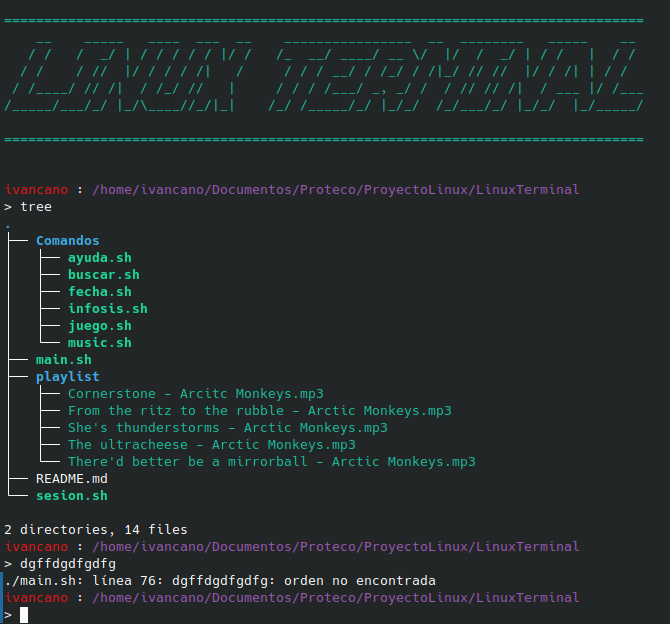
\includegraphics[scale=.4]{entrada.png} 
\end{figure}


\newpage
\subsection{Comando ayuda.sh}
Este comando es muy simple, proporciona la lista de comandos personalizados disponibles para que el usuario los pueda utilizar mientras mantiene activa su sesión.

\begin{figure} [H]
    \centering 
    \caption{Comando ayuda.sh}
    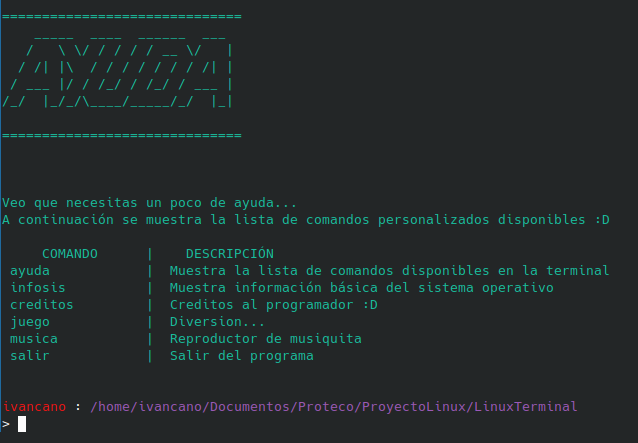
\includegraphics[scale=.6]{ayudaSH.png} 
\end{figure}

\subsection{Buscar archivos mediante un fichero}

El script buscar.sh nos permite buscar un archivo a partir de que el usuario ingresa su ruta en específico. Primero que nada verifiqué la existencia del directorio (ya que sino no se puede buscar a partir de ahí el archivo), y posteriormente como estoy trabajando como tal con cadenas de texto (las cuales son la ruta introducida por el usuario y el nombre del archivo a buscar) entonces ambas variables las concateno y terminé formando una ruta completa de un archivo. Si se logra encontrar al archivo, entonces quiere decir que ese archivo existe, mientras que sino entonces no se puede encontrar.

\begin{figure} [H]
    \centering 
    \caption{Comando buscar.sh}
    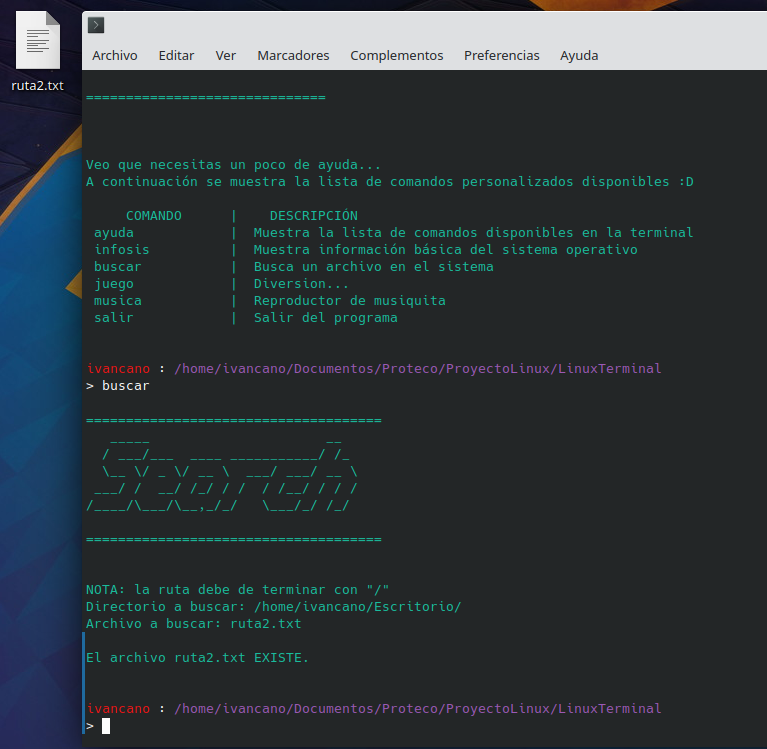
\includegraphics[scale=.6]{buscar.png} 
\end{figure}

\subsection{Fecha}
En el siguiente comando igual tenemos una lógica un tanto sencilla. Se me ocurrió pensar en algún archivo que tuviera la hora y fecha del sistema, ya que todo en linux es un archivo y por ende en algún lugar probablemente está. El directorio proc proporciona información de tiempo real en el sistema, descubrí que hasta me dice mucha información acerca de los componentes de mi computadora, y de hecho después me sería de gran utilidad para el comando infosis. La manera en la que obtengo la fecha y hora del sistema es accediendo al archivo rtc que significa Real Time Clock, que es un proceso que hace nuestro procesador y hardware para llevar un conteo del tiempo.

\begin{figure} [H]
    \centering 
    \caption{Fecha y hora}
    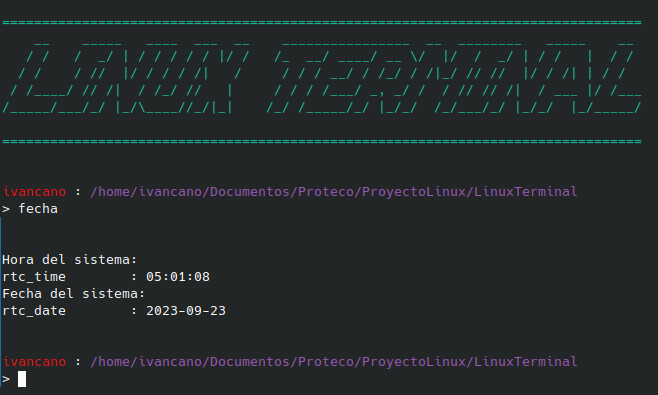
\includegraphics[scale=.5]{fecha1.png} 
\end{figure}

\subsection{Información del sistema}
Con ayuda de algunos archivos un tanto peculiares, obtuve información acerca de mi sistema operativo, en donde. Primero que nada utlicé awk para obtener la versión de la distribución de Linux y en donde imprimo solamente las 3 primeras columnas de información, que son las que me dan la información que yo requiero.\\
La arquitectura del sistema la obtuve con el comando arch, mientras que, como mencioné anteriormente en el apartado anterior, accedí a un archivo llamado meminfo en donde me muestra información acerca de la memoria del sistema, además de que utilicé el comando head para imprimir solamente la primera línea que era la que me interesaba. \\
Finalmente para el procesador, utilicé grepp, head y además cut, para que me mostrara la información de este a partir de los dos puntos y para que no me imprimiera la palabra completa.

\begin{figure} [H]
    \centering 
    \caption{infosis.sh}
    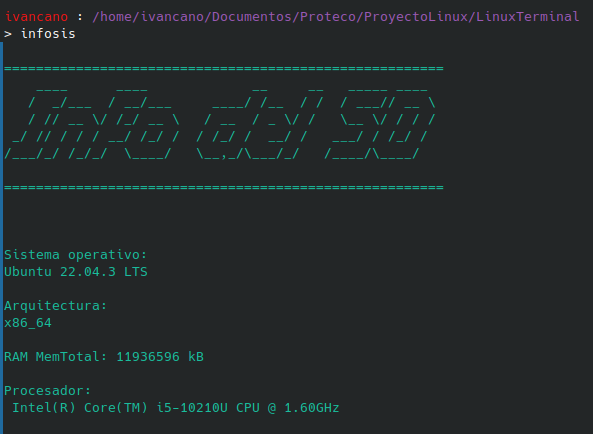
\includegraphics[scale=.5]{infosis.png} 
\end{figure}

\subsection{Juego}

Me decanté por elegir la opción del juego ahorcado. Sinceramente fue la parte que más me gustó programar, aunque en este script y en general en el desarrollo del proyecto tuve que investigar a fondo algunas sintaxis que no me había quedado claro. En este script podemos encontrar varias funciones que me ayudan a desplegar el muñequito de ahorcado, y que posteriormente me ayudan a mostrarlo en pantalla para hacer al juego más interactivo. \\

Posteriormente, defino lo que es un conjunto de palabras, en donde son las diferentes palabras que el usuario puede adivinar en el juego. También utilicé la función RANDOM para que pudiera acceder a cualquiera de los índices del arreglo, en donde en total cuento con 50 palabras registradas.\\

Yo quería que se mostrara en pantalla tanto el tablero como todas las coincidencias de una letra el momento de acertarla, por lo que decidí ocupar un segundo arreglo en donde lo incializo con guiones bajo a partir de la longitud que tenga la palabra a adivinar. Para mostrarlo en pantalla, utilicé el @ dentro de los corchetes del arreglo para mostrar todo su contenido, parecido a lo que comentaba en el arreglo de comandos personalizados en el main.\\

En el bucle principal, se ejectuan cada uno de los dibujitos del muñeco conforme a la cantidad de intentos restantes que le quedan al usuario. Además tambien verifico que solo pueda ingresar una sola letra.\\
Las variables de control booleanas fueron mis mejores amigas en este script, ya que primero la variable 'encontrado' me ayuda a verificar si la letra coincide con la palabra a adivinar, a partir de un recorrido de todos los caracteres en la palabra a adivinar. Si no se encontró ninguna coincidencia entonces se pierde un intento, pero si se encontró, entonces copia exactamente la misma letra en mi arreglo auxiliar y en exactamente el mismo índice, para que evidentemente concuerde la palabra.\\
Finalmente, utilzo una concatenación de cadenas para mostrar el avance del usuario y sus letras adivinadas, y además utilicé una variable de control más para saber si el arreglo auxiliar ya coincide con la palabra adivinar. Y asi sucesivamente hasta que el usuario la adivine o finalmente pierda.

\begin{figure} [H]
    \centering 
    \caption{Juego ahorcado}
    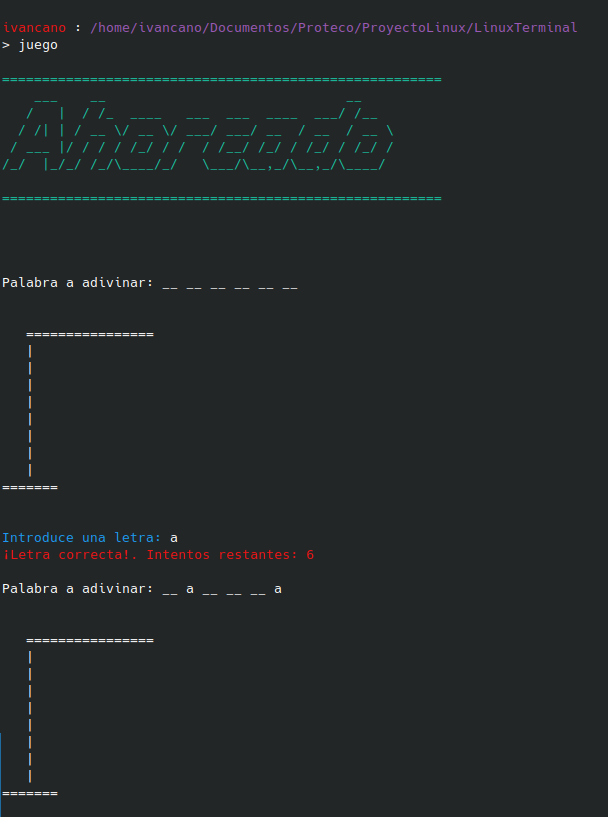
\includegraphics[scale=.7]{ahorcado1.png} 
\end{figure}

\begin{figure} [H]
    \centering 
    \caption{Palabra adivinada}
    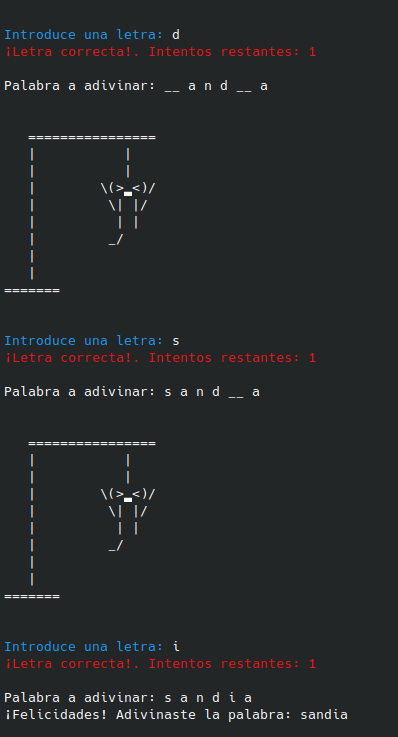
\includegraphics[scale=.7]{ahorcado2.png} 
\end{figure}

\subsection{Reproductor}
Finalmente, para el reproductor, se aprovecharon las herramientas de la aplicación mpg123 para poder manipular los archivos mp3. Me basé mucho en la idea de tener una playlist como archivo secundario, ya que ví que eso lo podía implementar mpg123 y me pareció una idea interesante.\\
El usuario puede escuchar su playlist ya sea mediante la playlist predeterminada del sistema, o bien, una playlist que se encuentre en alguna ruta de su sistema.\\
Algo muy imporante fue el uso del comando which para saber si mpg123 estaba ya instalado, de tal manera que aproveché el retorno de este comando con la variable de entorno \$?, esta me permite saber si el comando justo anterior que se ha ejecutado lo hizo con éxito o no. Si devuelve un valor igual a cero, entonces mpg123 si está instalado, ya que which se ejecutó correctamente, pero sino entonces lleva a cabo el proceso de instalación mediante sudo.\\

En dado caso de que ya esté instalado, entonces pasamos al menu principal en donde contamos con las 2 opciones que ya comenté anteriormente. \\
En este punto es importante mencionar el uso del archivo con extension .m3u, que es una especie de archivo de texto especial en donde mpg123 va a buscar archivos mp3 para reproducir, y este me va a servir como playlist para controlar la gestión de canciones en el reproductor. Con el comando find, a partir de la ruta predeterminada busco todas las coincidencias de archivos mp3 en la ruta default y direcciono su salida a la variable playlist, que es la que crea dicho archivo mencionado. De igual manera verifico que se haya creado correctamente y finalmente le pregunto al usuario de que manera quiere reproducir las canciones.\\
En caso de ingresar el usuario una ruta específica, entonces más validaciones para comprobar la existencia del directorio y del archivo pero en general sigue la misma lógica que el caso anterior.

\begin{figure} [H]
    \centering 
    \caption{Reproductor}
    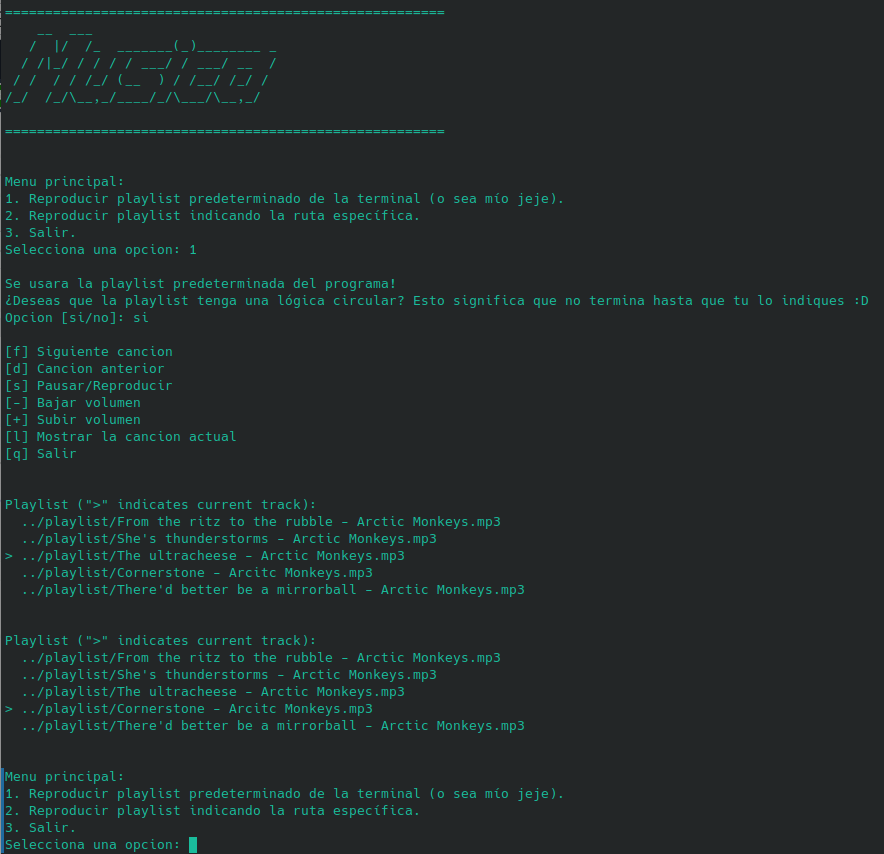
\includegraphics[scale=.6]{musica1.png} 
\end{figure}


\newpage
\section{Código anexado}
Nota: se exceptuaron los detalles estéticos como el ascii art para un mejor formato en la documentación.
\subsection{sesion.sh}
\begin{lstlisting}[language=sh, caption={Ventana de de inicio de sesión.}, label={lst:shellscript}, basicstyle=\small]
#!/bin/bash

echo
echo


while [ "$opcion" != 2 ]; do
    title
    echo
    echo
    echo "Selecciona una opcion:"
    echo "1. Iniciar sesion"
    echo "2. Salir"
    echo -n "Opcion: "

    read opcion

    case $opcion in 
    1)
        echo
        echo -n "Ingrese su nombre de usuario: "
        read username

        # Si se redirecciona algo al directorio "basura"
        # quiere decir que el usuario existe en el sistema.
        if getent passwd "$username" > /dev/null; then
            echo -n Ingresa tu contrasena:
            read -s password #Bandera -s para ocultar la entrada
            login=true
            if ! echo "$password" | su "$username" -c 'echo " "' 2> /dev/null; 
            then
                echo Upsss, contrasena incorrecta
                login=false
            fi

            if $login; then
                ./main.sh $username
            fi
        else
            echo "El usuario $username no existe en el sistema. 
            Registrate o haz algo, yo que se"
        fi
        ;;
    2)
        echo "Saliendo..."
        ;;
    *)
        echo "Opcion no valida"
        ;;
    esac
done


\end{lstlisting}

\subsection{main.sh}
\begin{lstlisting}[language=sh, caption={main del programa}, label={lst:shellscript}, basicstyle=\small]
#!/bin/bash

username=$1

# Funcion que se ejecuta cuando se recibe Ctrl+C o Ctrl+Z
function malo(){
    echo
    echo "EEEEeeeeEeeEeeEE A DONDE CREES QUE VAS? 
    Usa el comando salir o escribe ayuda."
    printf "> "
}

misComandos=(
    "ayuda"
    "fecha"
    "infosis"
    "buscar"
    "juego"
    "musica"
    "salir"
)

comando="a  "
title

while ! [[ $comando =~ salir ]]; do
    #echo $USER : $PWD
    trap 'malo' SIGTSTP
    trap 'malo' SIGINT
    printf "\033[31m$username\033[0m : \033[35m$PWD\033[0m"
    echo
    printf "> "
    read comando

    if grep -q "$comando" <<< "${misComandos[@]}"; then
        case $comando in
        ayuda)
            title
            ./Comandos/ayuda.sh;;
        infosis)
            ./Comandos/infosis.sh;;
        fecha)
            ./Comandos/fecha.sh;;
        buscar)
            ./Comandos/buscar.sh;;
        juego)
            ./Comandos/juego.sh;;
        musica)
            ./Comandos/music.sh;;
        salir)
            echo Vuelva pronto;;

        *)
            echo Opcion no valida, intenta de nuevo
            echo;;

        esac
    
    else
        $comando
        
    fi

 done

echo
echo

\end{lstlisting}


\subsection{ayuda.sh}
\begin{lstlisting}[language=sh, caption={Comando ayuda}, label={lst:shellscript}, basicstyle=\small]
#!/bin/bash

title

echo
echo Veo que necesitas un poco de ayuda...
echo A continuacion se muestra la lista de comandos personalizados disponibles
echo

echo "     COMANDO      |    DESCRIPCION    "
echo " ayuda            |  Muestra la lista de comandos disponibles en la terminal"
echo " infosis          |  Muestra informacion basica del sistema operativo"
echo " juego            |  Diversion..."
echo " musica           |  Reproductor de musiquita"
echo " salir            |  Salir del programa"


echo
echo -e "\e[0m"
\end{lstlisting}

\subsection{buscar.sh}
\begin{lstlisting}[language=sh, caption={Comando buscar}, label={lst:shellscript}, basicstyle=\small]
#!/bin/bash

title
echo "NOTA: la ruta debe de terminar con \"/\""
printf "Directorio a buscar: "
read ruta

printf "Archivo a buscar: "
read archivo

echo

if [ -d "$ruta" ]; then
    if [ -e "$ruta$archivo" ]; then
        echo "El archivo $archivo EXISTE."
    else
        echo "El archivo ingresado NO EXISTE."
    fi
else
    echo "La ruta ingresada no es un directorio o este no existe."
fi

echo
echo -e "\e[0m"

\end{lstlisting}

\subsection{fecha.sh}
\begin{lstlisting}[language=sh, caption={Fecha y hora}, label={lst:shellscript}, basicstyle=\small]

echo
echo
echo Hora del sistema:
grep rtc_time /proc/driver/rtc

echo Fecha del sistema:
grep rtc_date /proc/driver/rtc

echo
echo
\end{lstlisting}



\subsection{infosis.sh}
\begin{lstlisting}[language=sh, caption={Información del sistema}, label={lst:shellscript}, basicstyle=\small]
#!/bin/bash

ram=0

title
echo
echo Sistema operativo:
cat /etc/issue | awk '{print $1, $2, $3}'

echo Arquitectura:
arch

ram=$(cat /proc/meminfo | head -n 1)
printf "\nRAM " $ram
echo $ram

echo
echo Procesador:
cat /proc/cpuinfo | grep "model name" | head -n 1 | cut -d ":" -f 2-

echo
echo -e "\e[0m"

\end{lstlisting}


\subsection{juego.sh}
\begin{lstlisting}[language=sh, caption={Juego de ahorcado}, label={lst:shellscript}, basicstyle=\small]
#!/bin/bash

intentos_0(){
    echo "   ================"
    echo "   |           |"
    echo "   |           |"
    echo "   |        \(⁠>⁠ ⁠<⁠)/"
    echo "   |         \| |/"
    echo "   |          | |"
    echo "   |         _/ \_"
    echo "   |"
    echo "   |"
    echo "======="
}

intentos_1(){
    echo "   ================"
    echo "   |           |"
    echo "   |           |"
    echo "   |        \(⁠>⁠ ⁠<⁠)/"
    echo "   |         \| |/"
    echo "   |          | |"
    echo "   |         _/"
    echo "   |"
    echo "   |"
    echo "======="
}

intentos_2(){
    echo "   ================"
    echo "   |           |"
    echo "   |           |"
    echo "   |        \(⁠>⁠ <⁠)/"
    echo "   |         \| |/"
    echo "   |          | |"
    echo "   |         "
    echo "   |"
    echo "   |"
    echo "======="
}

intentos_3(){
    echo "   ================"
    echo "   |           |"
    echo "   |           |"
    echo "   |        \(⁠>⁠ <⁠)"
    echo "   |         \| |"
    echo "   |          | |"
    echo "   |         "
    echo "   |"
    echo "   |"
    echo "======="
}

intentos_4(){
    echo "   ================"
    echo "   |           |"
    echo "   |           |"
    echo "   |         (⁠>⁠ <⁠)"
    echo "   |          | |"
    echo "   |          | |"
    echo "   |          "
    echo "   |"
    echo "   |"
    echo "======="
}

intentos_5(){
    echo "   ================"
    echo "   |           |"
    echo "   |           |"
    echo "   |         (⁠>⁠ <⁠)"
    echo "   |         "
    echo "   |         "
    echo "   |         "
    echo "   |"
    echo "   |"
    echo "======="
}

intentos_6(){
    echo "   ================"
    echo "   |         "
    echo "   |         "
    echo "   |         "
    echo "   |         "
    echo "   |         "
    echo "   |         "
    echo "   |"
    echo "   |"
    echo "======="
}

# Define un conjunto de palabras
palabras=("manzana" "pera" "uva" "naranja" "platano" "sandia" "cereza" "fresa" 
          "kiwi" "melocoton"
          "londres" "inglaterra" "mexico" "argentina" "uruguay" "espana" "madrid" 
          "barcelona" "andorra" "canada"
          "messi" "ronaldo" "ronaldinho" "cristiano" "xavi" "iniesta" "modric" 
          "mbappe" "haaland" "puyol"
          "debian" "fedora" "gentoo" "ubuntu" "mint" "redhat" "centos" "linux" 
          "arch" "kali"
          "java" "c" "c++" "python" "javascript" "php" "ruby" "c#" 
          "basic" "fortran")

# Selecciona una palabra al azar del arreglo
indice=$(($RANDOM %50))
palabra="${palabras[$indice]}"

intentos=6
arr=()
n=${#palabra}
adivinado=false  # Variable para rastrear si la palabra ha sido adivinada

# Inicializa el array con guiones bajos
for ((i = 0; i < n; i++)); do
    arr[$i]="__"
done


title
echo
echo
echo "Palabra a adivinar: "${arr[@]}""

while [ $intentos -gt 0 ]; do
    echo
    echo

    if [ $intentos -eq 6 ]; then
        intentos_6
    elif [ $intentos -eq 5 ]; then
        intentos_5
    elif [ $intentos -eq 4 ]; then
        intentos_4
    elif [ $intentos -eq 3 ]; then
        intentos_3
    elif [ $intentos -eq 2 ]; then
        intentos_2
    else [ $intentos -eq 1 ]
        intentos_1    
    fi

    echo
    echo

    echo -n -e "\e[34mIntroduce una letra: \e[0m"
    read letra

    while [ ${#letra} != 1 ]; do
        echo -n -e  "\e[35mPor favor, introduce solamente una letra: \e[0m"
        read letra
    done

    encontrado=false

    for ((i = 0; i < n; i++)); do
        caracter="${palabra:$i:1}"
        if [ "$caracter" == "$letra" ]; then
            arr[$i]=$letra
            encontrado=true
        fi
    done

    if [ "$encontrado" == "false" ]; then
        intentos=$((intentos - 1))
        echo -e "\e[31mLetra incorrecta. Intentos restantes: $intentos\e[0m"
    else 
        echo -e "\e[31mLetra correcta!. Intentos restantes: $intentos\e[0m"
    fi

    resultado=""
    for char in "${arr[@]}"; do
        resultado="${resultado}${char} "
    done

    echo
    echo "Palabra a adivinar: $resultado"

    adivinado=true

    for char in "${arr[@]}"; do
        if [ "$char" == "__" ]; then
            adivinado=false
            break
        fi
    done

    if [ "$adivinado" == "true" ]; then
        break
    fi
done

if [ "$adivinado" == "true" ]; then
    echo "Felicidades! Adivinaste la palabra: $palabra"
else
    echo "Agotaste tus intentos. La palabra era: $palabra"
    intentos_0
fi

echo
echo


\end{lstlisting}


\subsection{music.sh}
\begin{lstlisting}[language=sh, caption={Reproductor}, label={lst:shellscript}, basicstyle=\small]
#!/bin/bash

title
rutaPredeterminada="../playlist/"
playlist="userPlaylist.m3u"  # Define la variable playlist aqui

controles(){
    echo
    echo "[f] Siguiente cancion"
    echo "[d] Cancion anterior"
    echo "[s] Pausar/Reproducir"
    echo "[-] Bajar volumen"
    echo "[+] Subir volumen"
    echo "[l] Mostrar la cancion actual"
    echo "[q] Salir"
    echo
}

#default recibe la ruta predeterminada del sistema para tomarla como playlist
default(){
    echo
    find "$1" -type f -name "*.mp3" > "$playlist"

    if ! [ -s "$playlist" ]; then
        echo La playlist no contiene archivos mp3 para ser creada! Agrega canciones plox.
        return
    else
        echo Se usara la playlist predeterminada del programa!
        echo "Deseas que la playlist tenga una logica circular? 
        Esto significa que no termina hasta que tu lo indiques :D"
        echo -n "Opcion [si/no]: "
        read circular

        while [[ "$circular" != "si" && "$circular" != "no" ]]; do
            echo -n "Por favor, solo introduce si o no: "
            read circular
        done

        controles
        if [ "$circular" = "si" ]; then 
            mpg123 -Z -q -@ "$playlist"
        else
            mpg123 -z -q -@ "$playlist"
        fi
        
    fi

    echo
}

rutaEspecifica(){
    echo
    echo -n "Introduce el directorio en donde tienes tu playlist (importante que termine en '/'): "
    read ruta

    if ! [ -d "$ruta" ]; then
        echo Error, la ruta ingresada no es un directorio.
        echo
    else
        echo
        find "$ruta" -type f -name "*.mp3" > "$playlist"

        if ! [ -s "$playlist" ]; then
            echo La playlist no contiene archivos mp3 para ser creada! Agrega canciones plox.
            echo
            
        else
            echo Se usara tu playlist ingresada :D
            echo "Deseas que la playlist tenga una logica circular? 
            Esto significa que no termina hasta que tu lo indiques :D"
            echo -n "Opcion [si/no]: "
            read circular

            while [[ "$circular" != "si" && "$circular" != "no" ]]; do
                echo -n "Por favor, solo introduce si o no: "
                read circular
            done

            controles
            if [ "$circular" = "si" ]; then 
                mpg123 -Z -q -@ "$playlist"
            else
                mpg123 -z -q -@ "$playlist"
            fi
        fi


    fi
}

which mpg123 > /dev/null 2>&1

if [ $? -eq 0 ]; then
    #mpg123 SI esta instalado
    opcion1=9


    while [ $opcion1 -ne 3 ]; do
        echo "Menu principal: "
        echo "1. Reproducir playlist predeterminado de la terminal (o sea mio jeje)."
        echo "2. Reproducir playlist indicando la ruta especifica."
        echo "3. Salir."
        echo -n "Selecciona una opcion: "
        read opcion1
        
        case $opcion1 in 
            1)
            default $rutaPredeterminada
            ;;
            2)
            rutaEspecifica
            ;;
            3)
            echo Regresa pronto :D
            rm $playlist
            exit 0
            ;;
            *)
            echo Opcion no valida, intenta de nuevo.
            ;;

        esac


    done
    
else
    #mpg123 NO esta instalado
    echo
    echo Upss, parece que no tienes mpg123 instalado.
    echo IMPORTANTE: solo para distribuciones basadas en debian
    echo -n Quieres instalar mpg123? Necesito una respuesta ahora "(si/no): "
    read op

    while [[ $op != "si" && $op != "no" ]]; do
        echo -n Introduce solamente "(si/no): " 
        read op
    done

    if [ $op = "si" ]; then
        echo Instalando mpg123...
        sudo apt update
        sudo apt install mpg123
        echo 
        mpg123 --version
    else
        echo Uy perdon, de regreso...
    fi
fi

echo
echo -e "\e[0m"
echo

\end{lstlisting}




\section{Conclusiones finales}
\begin{itemize}

    \item Fue un gran reto elaborar este proyecto, puse a prueba mis habilidades aprendidas en el curso. Al principio habían muchas cosas que yo no sabía, pero con un poco de paciencia salió la terminal y puedo decir que de cierta manera me gustó mi trabajo. La verdad si sentí el tiempo muy por encima pero fue por una cuestión de que me quedé sin buddy, de hecho por ese lado siento que algunas cosas mi terminal pudieron haber quedado mejor, pero aún así siento que aprendí muchísimo elaborando este proyecto. Lo más importante para mí fue que me gustaron las soluciones que propuse a los problemas que se me presentaron a la hora de diseñar el programa y de codificarlo, pero en resumidas cuentas siento que me esforcé y pude elaborar un buen trabajo.

    
\end{itemize}


\end{document}